\section{Evaluation}
\label{sec:evaluation}
\subsection{Questions and experimental scope}
The central claim is that one dependency-based organization method can adapt
to different butterfly computations. It does not require every optional
mechanism to help every workload. We therefore separate five questions.
Do automatically selected plans compete with specialized libraries?
When do individual mechanisms help, and can selection avoid their costs?
Does changing organization improve a fixed arithmetic core, including after
that core is replaced? How effectively does bounded search select plans?
Finally, do operator gains survive complete application execution?
External-library comparisons establish competitiveness on their sampled
workloads. Fixed-core controls separately test whether organization causes
a gain. Neither matching a closed-source library nor losing to it alone
isolates the contribution of hierarchical hybrid dataflow.

\textbf{Matched semantics.} Each operator row specifies arithmetic and
accumulation precision, direction, normalization, input/output order, shape,
batch, placement, and strides. Required conversions are timed and adapted
paths are identified. Integer comparisons require exact agreement. Current
floating-point records retain error distributions and reference-library
errors without an adopted acceptance threshold. Their timings are exploratory
performance observations, not completed numerical acceptance.

\textbf{Separate evidence populations.} The current screen uses a pinned
runtime on A100 80GB PCIe (SM80), CUDA 12.4, and PyTorch 2.5.1.
It contains 36 one-dimensional semantic requests across FFT, NTT, FWHT, subset
and superset zeta, and structured butterflies. A separate NTT extension
contains 12 forward/inverse requests and three process trials. We retain
older core, organization, and search experiments for their named hypotheses
and builds. Historical results are not inserted into missing current cells.
The artifact provides the unified absolute-latency table and a source ledger.
% Evidence: paper/evidence/EXPERIMENT_REUSE_20261012.json; current unified_report.

A separate October 17 review covers 66 requests, including rank-1/2/3/4/8
extensions: 29 integer requests agree exactly and all 37 floating outputs
have finite same-precision error distributions. Missing GPU comparisons and
floating acceptance remain explicit gaps. This independent build and population
supplement the evidence; they do not replace or enter the 36-plus-12 headline
statistics or the frozen figures below.

\subsection{Automatically selected operator performance}
\label{sec:rc2-results}
The screen exercises the public measured-selection path, rather than a
manually chosen resident kernel. Its timing protocol warms up ten complete
calls, captures twenty calls in a CUDA graph, and reports the median of seven
event-timed replays divided by twenty. All applicable libraries use this
protocol. Compilation, plan selection, and reference checking are excluded.
The 36-point screen has one process trial per request, whereas the NTT
extension independently repeats the selected mapping in three processes.
Replay samples are not treated as independent process trials.

\begin{figure*}[t]
\centering
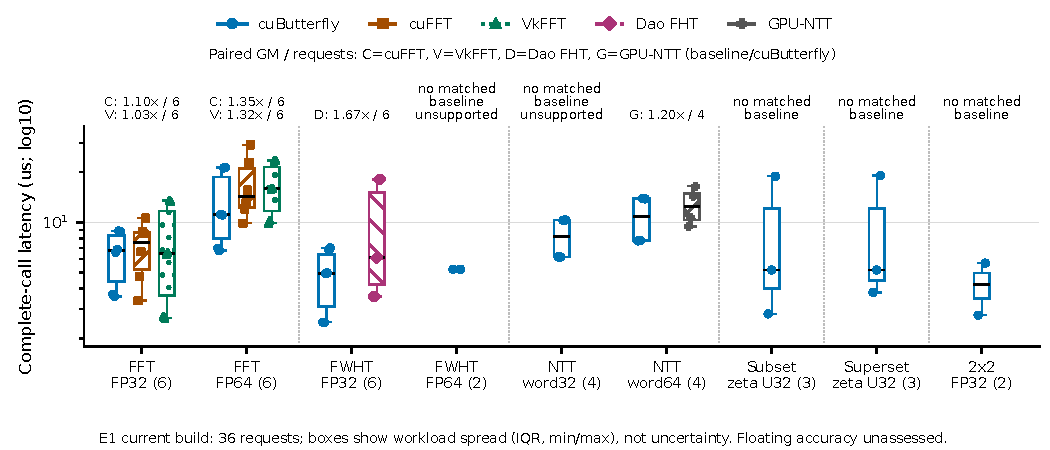
\includegraphics[width=.98\textwidth]{figures/principle_e1_latency.pdf}
\caption{Current A100 80GB operator screen. Absolute complete-GPU-call
latencies use the same graph-replay timing protocol. Each point is one
semantic request; boxes describe the sampled workload distribution, not
measurement uncertainty. Operator and precision groups remain separate.
Paired speedups are baseline latency divided by \system{} latency and are
reported separately for each competitor. Empty comparisons indicate missing
matching implementations, not wins. Floating accuracy remains under review.}
\label{fig:rc2-absolute-throughput}
\end{figure*}

Figure~\ref{fig:rc2-absolute-throughput} separates the performance of each
arithmetic family. The six FP32 FFT requests yield a geometric mean of
1.103$\times$ over cuFFT with four wins; the six FP64 requests yield
1.353$\times$ with six wins. Against VkFFT, the respective means are
1.029$\times$ and 1.325$\times$, with two and six wins.
The six FP32 FWHT requests yield 1.667$\times$ over the matched Dao interface.
These observations establish competitiveness on the sampled requests, while
preserving FFT losses rather than inferring uniform superiority from a mean.

The NTT extension crosses $N\in\{4096,65536\}$ with $B\in\{1,16,256\}$
and both directions using the same word64 field and natural-order contract.
All 12 requests pass exact checking and beat GPU-NTT, with ratios from
1.029$\times$ to 1.615$\times$ and a 1.285$\times$ geometric mean.
Its four batch-one requests are repeated controls and are not pooled with
the earlier screen. Word32 NTT, FP64 FWHT, zeta, and structured requests
retain their measured times but lack matching external comparisons here.
Thus support for these families is not itself evidence of external speedup.

\subsection{Ablation I: mechanisms and adaptive organization}
\label{sec:component-ablation}
The mechanism study asks when retaining data or overlapping work compensates
for its resource and orchestration costs. Two controls answer different
questions. A fixed-core, fixed-condition toggle explains a mechanism.
Disabling that mechanism and \emph{repeating search under the same budget}
tests its contribution to the automatically selected implementation.
Our controls include fixed-condition toggles and a newer bounded
cross-operator restricted-search study. A negative toggle result identifies
an applicability boundary, not a failure of the common representation.

For the current FFT factor-streamed control at $N=256$, $B=16384$, enabling
slice overlap changes native-core latency from 127.560 to 132.346~$\mu$s and
imported-core latency from 126.331 to 130.957~$\mu$s. Both variants still
launch three kernels, and measured L2 traffic changes by less than 0.2\%.
The imported core uses fewer registers per kernel, but its whole-call gain
is only about 1\%. These results motivate choosing overlap from its complete
cost, rather than always enabling it or treating lower register count as
sufficient evidence of higher throughput.

The October 17 selector study repeats search with stage overlap, resident
fusion, or successor layout disabled, using eight scheduled candidates per
space for FFT ($N=16384,B=16$), FWHT and NTT ($N=16384,B=4$).
FFT and FWHT timing differences are small; NTT restricted-search regret is
0.7\% for resident fusion and 2.9\% for successor layout, with overlap within
measurement noise. The latter NTT pair accepts eight restricted candidates
versus six unrestricted candidates because two unrestricted mappings fail
legality checks. These traces establish an executable restriction protocol
and its candidate-population effects, not a stable universal mechanism gain;
independent winner confirmation and broader requests remain necessary.

\begin{table}[t]
\centering\small
\caption{Current FFT core/overlap diagnostic. Ordinary latency is the median
of three process trials; counters are from separate NCU kernel captures.
Registers list the three kernels in execution order. L2 totals are decimal
MB, not an average bandwidth or a complete application traffic estimate.}
\label{tab:component-counters}
\begin{tabular}{@{}llrrl@{}}
\toprule
Core & Overlap & $\mu$s & L2 MB & Registers\\\midrule
Native & Off & 127.560 & 201.83 & 61/61/63\\
Native & On & 132.346 & 201.57 & 61/61/63\\
Imported & Off & 126.331 & 201.48 & 52/52/36\\
Imported & On & 130.957 & 201.54 & 52/52/36\\
\bottomrule
\end{tabular}
\end{table}

The earlier layout/depth and batch controls reach the same qualitative
conclusion. Writer-aligned layout loses in its three tested pairs, while
greater resident depth wins in three pairs. Pipeline batching loses to bulk
in 27/27 A100 80GB comparisons. In a matched $N=4096$, $B=64$ example,
ordinary timing is 29.266~$\mu$s for bulk and 45.636~$\mu$s for the pipeline.
Nsight Systems observes overlap, but the pipeline issues eight launches per
call instead of two. The limitation is the balance between useful overlap
and fragmentation, not whether overlap can be expressed.

\textbf{Counter boundaries.} NCU counters describe sampled kernels;
ordinary timing measures performance. Copies are listed separately. For
example, the fixed-mapping Dao FWHT diagnostic contains a 2~MiB device copy
outside its NCU kernel byte totals. We do not interpret those totals as
complete-call traffic. The deliberately underfilled stagewise diagnostics
are likewise excluded from claims about a well-tuned baseline. The artifact
retains their registers, shared-memory conflicts, traffic, and wait metrics.

A separate current-build six-request control changes stage partitioning for
FFT, FWHT, and word64 NTT at $N=4096,B=4$ and $N=262144,B=1$.
Stagewise-over-resident-8 ratios range from 10.87$\times$ to 22.44$\times$.
The paired FWHT profile records 18 versus three kernels at the larger shape.
These large ratios expose the launch and global-boundary cost of the
stagewise control, not an optimized external-library comparison.

\subsection{Ablation II: organization benefits at fixed core}
\label{sec:core-organization}
Whole-library improvements could otherwise be explained by a larger
collection of arithmetic kernels. To isolate organization, we reuse a
four-cell experiment that embeds the same 16-point arithmetic leaf in two
execution organizations, then repeats the comparison with another leaf.
The core axis selects native register arithmetic or cuFFTDx Thread.
The organization axis selects stagewise HBM exchange or a resident two-stage
prefix; later stages retain the same global-stage template.

\begin{figure}[t]
\centering
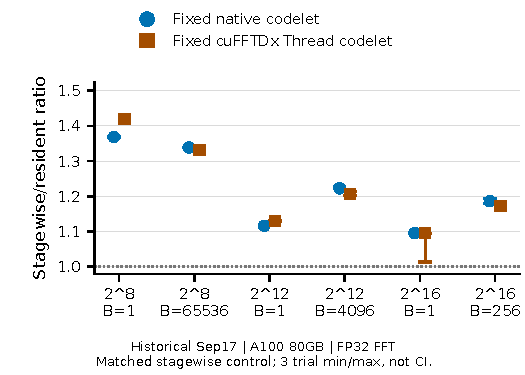
\includegraphics[width=\columnwidth]{figures/principle_core_organization.pdf}
\caption{Historical A100 80GB fixed-leaf organization control. Each series
keeps its arithmetic leaf fixed and compares stagewise-HBM with
resident-prefix-2 execution. Six workloads cross three lengths with latency
and throughput batches. Ratios use three-trial median latencies; error bars
show paired trial ranges, not confidence intervals. Values above one favor
residency. Both leaf implementations benefit. This independent
mechanism executable is distinct from the current public-library cohort.}
\label{fig:core-organization}
\end{figure}

Six FP32 workloads each have four cells and three trials, producing 72 rows.
Each trial uses complete-batch reference checks, 10,000 warmups, and 100
repetitions. Residency improves all six workloads for both cores, with
geometric means of 1.217$\times$ and 1.221$\times$
(Figure~\ref{fig:core-organization}). Replacing the core at fixed organization
contributes 1.042$\times$ for stagewise and 1.046$\times$ for resident
execution. The organization benefit is therefore separately visible within
each core, rather than being attributed to core substitution.

The fixed object is the arithmetic leaf, not the entire GPU kernel.
For $N=256$, $B=1$, stagewise and resident execution launch 16 and 256
threads respectively. Shared storage, parallelism, and launch count are
part of the organization treatment; the stage-zero wrappers also differ in
source. We therefore make no claim of identical wrapper instructions or
launch geometry. A separate A100 40GB replication retains same-core
organization gains of 1.226$\times$ and 1.231$\times$; its trials are not
pooled with the 80GB results.

\textbf{Prefetch transfer across local cores.}
A newer A100 80GB FP64 control fixes $N=65536$, $B=16$, two 256-point
factor transforms, four parallel local transforms per CTA, and 16 elements
per thread. Both the repository's auditable register core and cuFFTDx Block
use the same factor execution template and writer-aligned handoff.
Only the number of tile groups consumed per CTA and the prefetch depth vary.
Figure~\ref{fig:factor-organization} reports every tested organization and
the matched complete cuFFT call.

\begin{figure}[t]
\centering
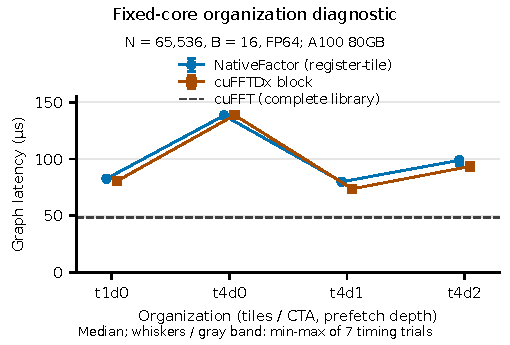
\includegraphics[width=\columnwidth]{figures/factor_organization_20261025.pdf}
\caption{Fixed-core organization diagnostic on A100 80GB, FP64,
$N=65536$, $B=16$. For example, \texttt{t4d1} denotes four consecutive
tile groups per CTA and prefetch depth one. Markers show complete-Graph median latency and whiskers
show the range of seven rounds in one process, not independent-process
confidence intervals. One-step prefetch helps both cores; deeper prefetch
regresses, and complete cuFFT remains faster.}
\label{fig:factor-organization}
\end{figure}

At four tile groups per CTA, one-step prefetch reduces native-core latency
from 138.377 to 79.974~$\mu$s and cuFFTDx latency from 138.684 to
73.762~$\mu$s, giving 1.730$\times$ and 1.880$\times$.
The faster one-tile synchronous alternative takes 82.671 and
80.657~$\mu$s, so gains against that alternative are only
1.034$\times$ and 1.093$\times$. Depth two regresses for both cores.
cuFFT takes 48.503~$\mu$s and remains faster on this request.
All outputs are finite and relative L2 errors against CPU FP64 are below
$7.4\times10^{-16}$, without introducing a numerical acceptance threshold.
This control demonstrates conditional prefetch benefits across cores.
It does not compare the full method against either core's original library
organization, establish automatic selection, or supersede the historical
leaf-residency experiment.

A historical cross-arithmetic study holds the shared-iterative arithmetic
core and physical groups fixed while changing local stage partitioning.
At $N=4096$ and batches 1/1024, FWHT improves by 1.137/1.302$\times$ and
word64 NTT by 1.073/1.091$\times$. This extends evidence for same-core
organization gains across arithmetic families. It is not a two-core factorial
for either family, nor a change to the groups' HBM boundaries. Its lowering
changes group-local shared/register exchange and synchronization.
Completing that crossing for FWHT, NTT, zeta, and structured
butterflies is a separate coverage requirement; radix labels alone do not
establish interchangeable core implementations.

New current-build controls separately compare shared-core FWHT stage
partitioning, temporal FWHT radix-2/radix-4 cores, and specialized NTT
radix-2/vector-radix-4 cores. All six rows pass their recorded correctness
checks. Their different shapes and lowering support domains do not form a
two-core/two-organization crossing, so the wider factorial gap remains.

\subsection{Coverage, selection, and preparation cost}
\label{sec:selection-evaluation}
The common interface combines semantic dimensions instead of assigning a
separate evaluation protocol to each named variant. The present screen does
not exhaust their Cartesian product. Earlier precision, inverse, layout,
and multidimensional records remain separately identified coverage evidence.
The broader historical RC2 FFT distribution reports 21/36 wins and a
1.031$\times$ geometric mean over cuFFT, and 13/20 wins with 1.026$\times$
over VkFFT. Those builds and workloads differ from the current screen;
the stronger current means are not a like-for-like version improvement.
The RC2 distribution and 27-point contiguous FFT scaling study remain
separate artifact records.
Likewise, the A100 40GB replication is a same-architecture experiment;
historical V100 results do not establish same-version cross-architecture
portability.

Selection is evaluated against the best \emph{measured} candidate, with
candidate coverage, ordering, and preparation cost reported independently.
In an earlier 16-candidate replay, informed policies find the pool best at
budgets four, eight, and sixteen. Random search's mean selected-time to
pool-best ratios are 1.486, 1.002, and 1.000 for FFT, and 2.228, 1.074,
and 1.000 for NTT. The stage-service policy has no covered priors in this
replay and falls back to structural ordering. These results support
finite-pool prioritization, not calibrated prediction accuracy, global
optimality, or online tuning cost.

Install-time service calibration and post-install tuning are implementation
stages of this selection process. Their presence does not establish that
every lowering consumes the resulting model. In the current implementation,
native multidimensional plans use complete-plan measurement and a persistent
cache separately from the rank-one calibrated registry. The application
experiment explicitly tunes those plans outside timing and requires cache
replay during measurement. Search, compilation, first use, and steady-state
execution remain separate costs. The bounded restricted-search study above
adds current cross-operator evidence; independent winner timing and online
preparation costs remain necessary for the adaptive-selection claim.

\subsection{Complete applications and batch scaling}
\label{sec:application-evaluation}
Finally, we test whether the selected organization remains useful after
integration. FFT image filtering and FNO/NeuralOperator cover image-domain
and neural spectral workloads; QuaRot/Llama covers FWHT, and HEonGPU CKKS
supplies the NTT application~\cite{neuraloperatorcode,quarotcode,heongpucode}.
All variants use identical inputs, weights or keys, and precision. The timed
boundary includes surrounding GPU work, required packing, conversions,
and synchronization. Model loading, compilation, reusable plans,
and first use are excluded and recorded separately.

\begin{figure*}[t]
\centering
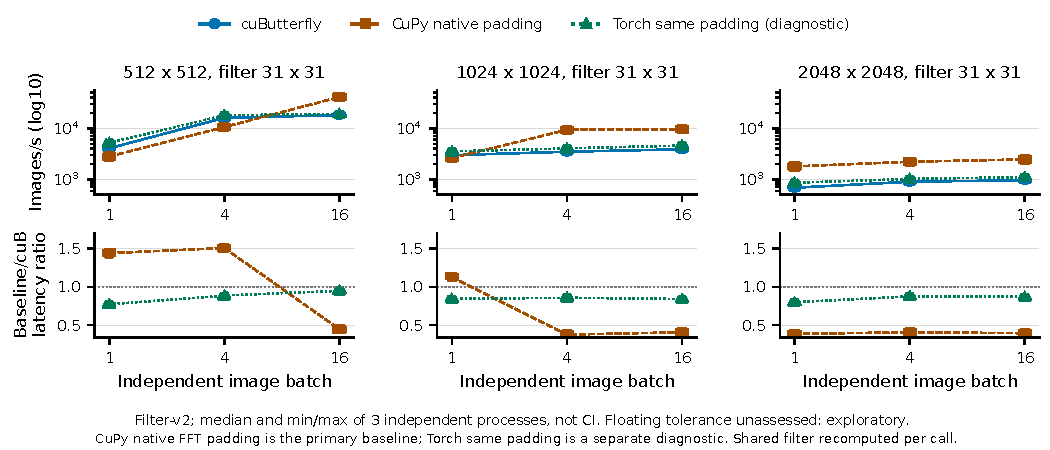
\includegraphics[width=.98\textwidth]{figures/principle_application_throughput_ratio.pdf}
\caption{Complete FP32 image-filter calls on A100 80GB, using independent
images and the same $31\times31$ filter at each batch. Each size has three
independent process trials with rotated method order. CuPy uses its native
FFT padding; the same-padding PyTorch/cuFFT path is a separate diagnostic.
All required padding, transforms, multiplication, and cropping are timed.
These are measured exploratory results, with floating error reported and
no adopted acceptance threshold. Increasing batch improves throughput but
does not guarantee a better ratio against the competitor. Error bars show
the range across three process trials, not a confidence interval.}
\label{fig:application-batch}
\end{figure*}

The filter matrix crosses image edges 512, 1024, and 2048 with batches one,
four, and sixteen. Each call recomputes one shared filter spectrum; none of
the backends uses a cached filter to gain an artificial advantage. After
untimed tuning, every \system{} plan in all three process trials replays its
persistent cache. The maximum observed relative $L_2$ error is
$5.76\times10^{-7}$ for \system{} and $3.95\times10^{-7}$ for CuPy.

Figure~\ref{fig:application-batch} preserves the unfavorable cases.
\system{} wins three of nine comparisons, including 1.448$\times$ and
1.516$\times$ for 512-edge images at batches one and four. At batch sixteen,
the same size reaches about 18,109 images/s versus CuPy's 40,812 images/s.
The larger-image cases also expose a gap. \system{} currently pads to powers
of two, whereas CuPy selects smaller supported FFT extents; the same-padding
diagnostic remains faster as well. Extra transform work is therefore one
boundary, but cannot explain the entire difference. The data do not support
claiming that more independent inputs alone eliminate integration costs.

An independent October 18 fixed-filter Graph cohort changes that contract:
all three backends cache the filter spectrum before timing and use matching
fast padding ($1080^2$ or $2100^2$), with $B=16$ and a $31^2$ filter.
For image edges 1024/2048, complete-call medians are 1.406/5.731~ms for
\system{}, 1.500/5.904~ms for CuPy, and 1.533/6.007~ms for Torch/cuFFT.
Timing includes input device copies, image padding, transforms, multiplication,
cropping, and independent output copies; setup and capture are excluded.
Changed/restored-input and output-lifetime checks pass. These five-sample,
single-process observations retain floating error reports without an adopted
acceptance threshold. They show gains for these two cached-filter requests;
the nine-point recomputed-filter cohort and its losses remain separate.

We also measure a 2D periodic spectral Poisson endpoint at $N=2048$, $B=16$,
FP32, with the same complete copy boundary for all backends. The adaptive xD
plan measures axis candidates after the budget repair and replays them through
a CUDA Graph. Figure~\ref{fig:application-poisson} shows twenty steady-state
calls in one process, not independent process trials.

\begin{figure}[t]
\centering
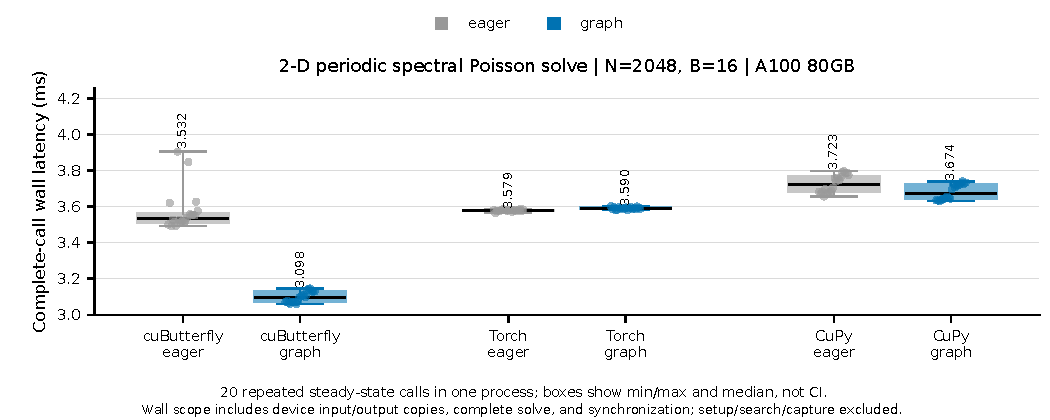
\includegraphics[width=.99\columnwidth]{figures/principle_application_poisson_endpoint.pdf}
\caption{Measured 2-D periodic spectral Poisson endpoint on an A100 80GB at
$N=2048$, $B=16$. The boundary includes device copies, both FFTs, the
frequency-domain multiplier, and synchronization; setup, search, and capture
are excluded. Boxes contain twenty steady-state calls from one process and
labels show medians.}
\label{fig:application-poisson}
\end{figure}

Graph medians are 3.098~ms for \system{}, 3.590~ms for Torch, and 3.674~ms
for CuPy, giving 1.159$\times$ and 1.186$\times$ against the two baselines.
The adaptive plan uses two fused axis launches per direction and removes the
four serialized transpose kernels and separate scale kernel of the fallback.
This measured endpoint remains separate from the nine-point image-filter cohort.

\begin{table}[t]
\centering\small
\caption{Other completed application records, kept separate from the filter
cohort. Times are milliseconds per complete call. QuaRot uses two process
trials with identical random weights; FNO uses its separately recorded
three-trial prior-day cohort. CKKS uses a separate cohort below.}
\label{tab:applications}
\begin{tabular}{@{}lrrrl@{}}
\toprule
Application & $B$ & \system{} & Baseline & Backend\\\midrule
QuaRot 512/32 & 1 & 2533.32 & 2482.87 & Dao\\
FNO $64^2$ & 4 & 2.946 & 2.783 & cuFFT\\
FNO $128^2$ & 4 & 2.965 & 2.810 & cuFFT\\
\bottomrule
\end{tabular}
\end{table}

The repaired QuaRot path reproduces the baseline outputs exactly for the
measured random-weight model, but its complete prefill-plus-decode call is
about 2\% slower (Table~\ref{tab:applications}). It uses the SDPA fallback,
not a FlashAttention comparison. FNO also remains slower. These records
measure implementation consistency and execution, not trained-model quality.
QuaRot batch expansion remains separate unfinished coverage.

The October 19 CKKS study tests whether batching corresponding NTT stages
across independent ciphertexts carries organization gains into complete
operations. It covers key switching, square/relinearize/rescale, that chain
followed by key switching, and slot rotation, at $B=1,8,32$.
All 36 configurations and 144 execution paths produce elementwise-identical
ciphertexts. Four paths share inputs and keys: native loop, \system{} loop,
native-core batch, and \system{} batch. Both batched paths share graph
organization and gather/scatter; the native batched control is constructed
by this integration, not an upstream batch API.

\begin{table}[t]
\centering\small
\caption{Independent CKKS complete-Graph cohort. Geometric mean ratios are
baseline over \system{} batch; above one favors \system{}. Each row contains
four $B=1$ and eight $B=8,32$ configurations. Loop and batch baselines remain
separate. All graph packing, NTT, writeback, and non-NTT work is timed.}
\label{tab:ckks-batch}
\begin{tabular}{@{}lrrr@{}}
\toprule
Method / $N$ & $B=1$ loop & $B>1$ loop & $B>1$ batch\\\midrule
I / 16384 & 0.723 & 1.862 & 1.124\\
I / 65536 & 0.884 & 1.195 & 1.143\\
II / 16384 & 0.723 & 1.755 & 1.128\\
\bottomrule
\end{tabular}
\end{table}

All 24 multi-ciphertext configurations beat both native controls, whereas
forced batching loses for all 12 $B=1$ configurations. Two large-$N$ rotation
cases also prefer \system{}'s own loop to its batch path. Application-level
loop/batch selection is therefore still required; these measurements do not
establish an automatic policy. Timing uses twenty rotated rounds of ten
Graph replays, with thermal guards and default dynamic clocks; setup, search,
capture, encryption, and checking are excluded. The context uses
$Q=[50,40,40]$, $P=[50]$ or $[50,50]$, scale $2^{40}$, and
\texttt{sec\_level=none}. These are complete FHE operations and short chains,
not full bootstrap or production-security validation. Request-level RNS
tuning remains distinct from installation-model integration. Thus sampled
application gains now complement the operator and organization evidence,
while broader cross-core, application, and platform coverage remains open.
